\chapter{Implementation}
\section{RAG Chatbot}
    \subsection{Chatbot Interface}
        The chatbot interface was developed using the \texttt{Streamlit} library, which provides a simple and interactive way to create web applications. The interface allows users to interact with the RAG chatbot by entering a question in the input field and receiving the corresponding answer from the model. The chatbot interface was designed to be user-friendly and intuitive, enabling users to easily communicate with the chatbot and obtain relevant information.
        \begin{figure}[H]
            \centering
            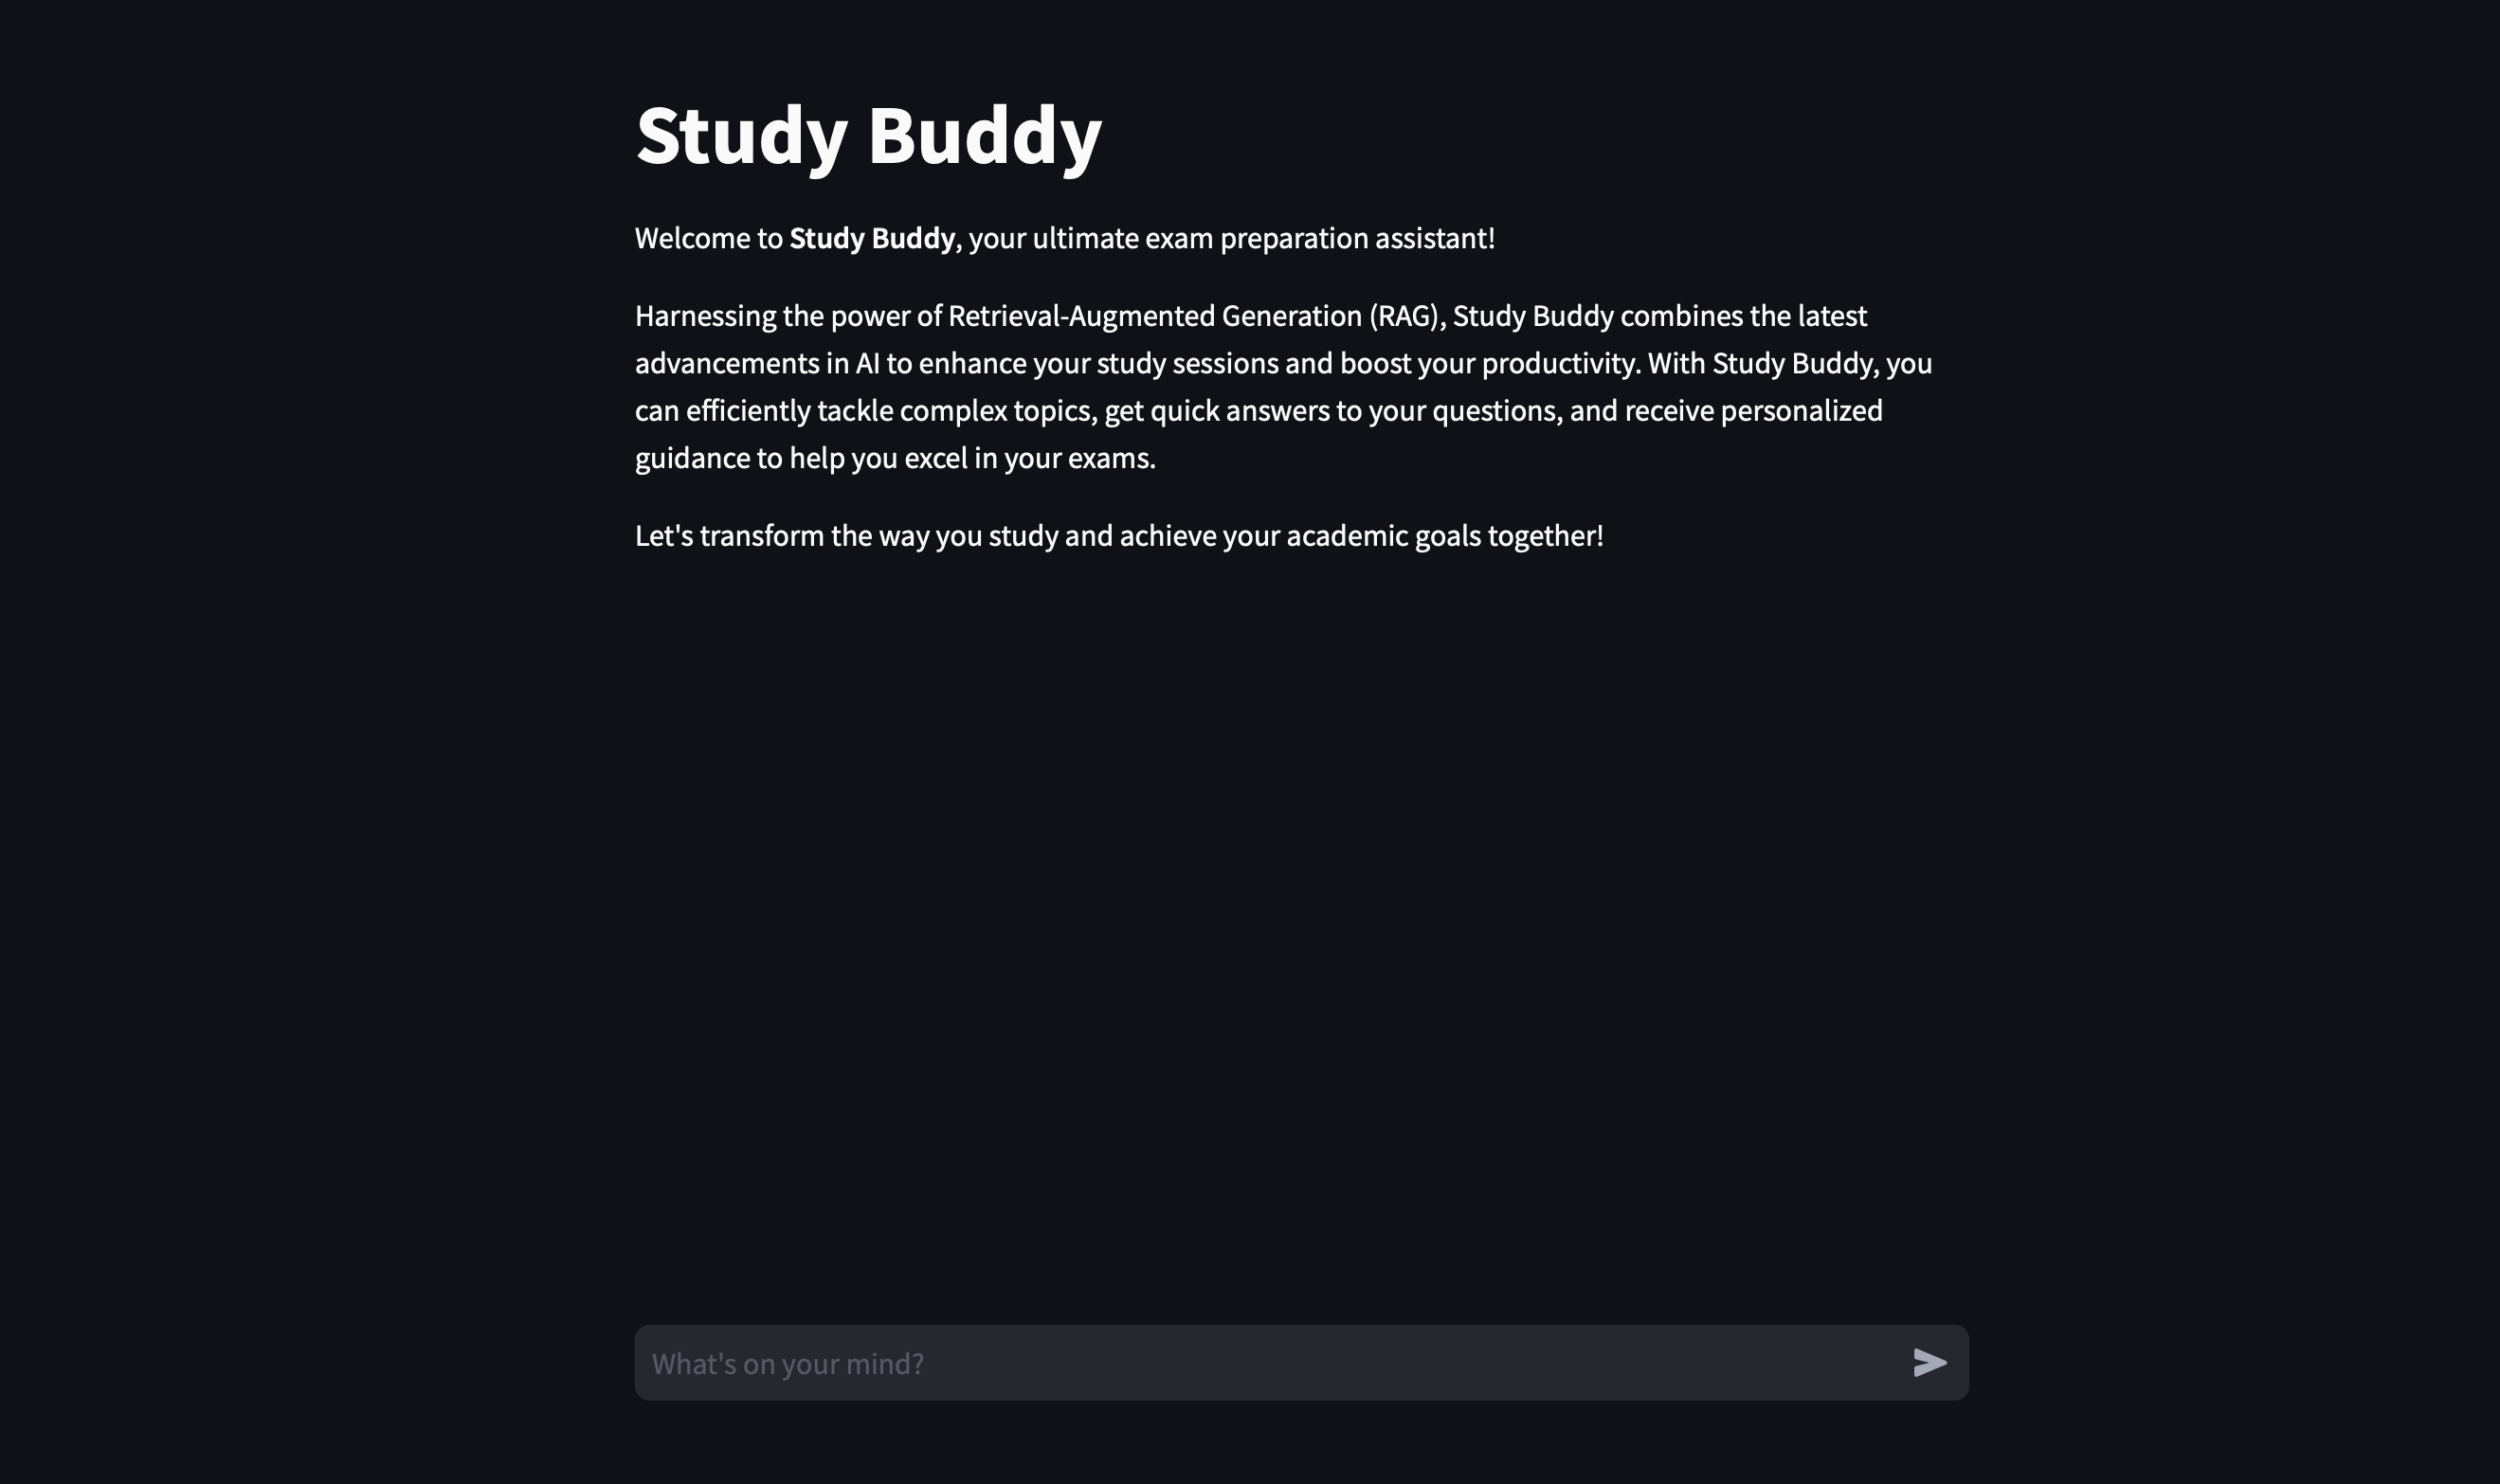
\includegraphics[width=0.8\textwidth]{figs/interface.png}
            \caption{RAG Chatbot Interface}
            \label{fig:chatbot_interface}
        \end{figure}
            
            The chatbot interface displays a title, description and input field for user queries using the \texttt{st.title}, \texttt{st.markdown} and \texttt{st.chat\_input} functions respectively. The title introduces the chatbot as "Study Buddy," while the description provides an overview of the chatbot's capabilities and features. By using the \texttt{Streamlit} library, the chatbot interface can be created by just a few lines of code.

    \subsection{Generator Component}
        The generator component of Study Buddy was implemented using the \texttt{Langchain} library, which provides ready-to-use methods to call OpenAI's GPT-4 model. Streamlit reruns the code in the \texttt{app.py}-file everytime a user interacts with the chatbot. The following code snippets show how the generator calls the GPT-4 model and generates responses to user queries.
        \begin{listing}[H]
\begin{minted}[fontsize=\footnotesize]{python}
from langchain_openai import ChatOpenAI
# Cache OpenAI Chat Model for reuse
@st.cache_resource()
def get_chat_model():
    return ChatOpenAI(
        temperature=0.3,
        model='gpt-4',
        streaming=True,
        verbose=True
    )
chat_model_instance = get_chat_model()
\end{minted}
            \caption{Caching the OpenAI Chat Model}
            \label{listing:Cache_Chat_Model}
            \end{listing}
            
            \begin{listing}[H]
\begin{minted}[fontsize=\footnotesize]{python}
# Generate response using the OpenAI Chat Model
input_data = RunnableMap({
        'context': lambda x: retriever_instance.get_relevant_documents(x['question']), # Retrieve relevant documents
        'question': lambda x: x['question']
    })
response_chain = input_data | chat_prompt | chat_model_instance
generated_response = response_chain.invoke({'question': user_question}, config={'callbacks': [ResponseStreamHandler(response_placeholder)]})
assistant_answer = generated_response.content

# Display the final response
response_placeholder.markdown(assistant_answer)
\end{minted}
            \caption{Generating Responses using the OpenAI Chat Model}
            \label{listing:Generate_Responses}
            \end{listing}
            


\section{Case Study}

    \subsection{Importing the Model}
        The BART-base model was imported from the Hugging Face platform using the \texttt{transformers} library.
        \begin{listing}[H]
            \begin{minted}[fontsize=\footnotesize]{python}
model_checkpoint = "facebook/bart-base"
model = AutoModelForSeq2SeqLM.from_pretrained(model_checkpoint)
            \end{minted}
            \caption{Importing the BART-base model}
            \label{listing:Importing_BART}
        \end{listing}
    
        \subsection{Dataset Preprocessing}

The SamSum dataset was imported and preprocessed to facilitate the training and evaluation of the BART-base model. The dataset comprises conversations crafted and documented by linguists proficient in English, which were subsequently annotated with summaries. The preprocessing steps included tokenization, truncation, and padding to ensure uniform input sizes for the model.

\subsubsection{Importing the Dataset}

First, we imported the necessary libraries and loaded the SamSum dataset using the \texttt{datasets} library:

\begin{listing}[H]
\begin{minted}[fontsize=\footnotesize]{python}
from datasets import load_dataset

raw_datasets = load_dataset("samsum")
\end{minted}
\caption{Loading the SamSum dataset}
\label{listing:Loading_SamSum}
\end{listing}

The \texttt{load\_dataset} function fetches the SamSum dataset, which contains dialogues and their corresponding summaries.

\subsubsection{Setting Maximum Lengths}

To ensure that the input and target sequences fit within the model's constraints, we set the maximum lengths for input and target sequences:

\begin{listing}[H]
\begin{minted}[fontsize=\footnotesize]{python}
max_input_length = 512
max_target_length = 128
\end{minted}
\caption{Setting maximum lengths for inputs and targets}
\label{listing:Max_Lengths}
\end{listing}

Here, \texttt{max\_input\_length} is set to 512 tokens and \texttt{max\_target\_length} is set to 128 tokens, which are reasonable lengths for dialogues and summaries respectively.

\subsubsection{Preprocessing Function}

Next, we defined a preprocessing function to tokenize the inputs and targets. This function truncates and pads the sequences to the specified maximum lengths:

\begin{listing}[H]
\begin{minted}[fontsize=\footnotesize]{python}
def preprocess_function(examples):
    inputs = [doc for doc in examples["dialogue"]]
    model_inputs = tokenizer(inputs, max_length=max_input_length, truncation=True)

    # Setup the tokenizer for targets
    with tokenizer.as_target_tokenizer():
        labels = tokenizer(examples["summary"], max_length=max_target_length, truncation=True)

    model_inputs["labels"] = labels["input_ids"]
    return model_inputs
\end{minted}
\caption{Defining the preprocessing function}
\label{listing:Preprocess_Function}
\end{listing}

This function performs the following steps:
\begin{itemize}
    \item Tokenizes the dialogue texts.
    \item Sets up the tokenizer for the target summaries.
    \item Tokenizes the summaries and adds them to the \texttt{model\_inputs} dictionary as labels.
\end{itemize}

\subsubsection{Applying the Preprocessing Function}

Finally, we applied the preprocessing function to the entire dataset using the \texttt{map} method, which processes the dataset in batches:

\begin{listing}[H]
\begin{minted}[fontsize=\footnotesize]{python}
tokenized_datasets = raw_datasets.map(preprocess_function, batched=True)
\end{minted}
\caption{Applying the preprocessing function to the dataset}
\label{listing:Tokenized_Datasets}
\end{listing}

The \texttt{map} method applies the \texttt{preprocess\_function} to each example in the dataset, ensuring that all dialogues and summaries are properly tokenized, truncated, and padded. This results in a tokenized dataset ready for training and evaluation with the BART-base model.

    \subsection{Finetuning the Model}
        The model was then fine-tuned on the SamSum dataset for dialogue summarization tasks.
        \begin{table}[h!]
            \centering
            \resizebox{\textwidth}{!}{%
                \begin{tabular}{cccccccc}
                    \toprule
                    \textbf{Epoch} & \textbf{Training Loss} & \textbf{Validation Loss} & \textbf{Rouge1} & \textbf{Rouge2} & \textbf{Rougel} & \textbf{Rougelsum} & \textbf{Gen Len} \\
                    \midrule
                    0 & 1.81 & 1.54 & 47.39 & 24.45 & 40.03 & 43.77 & 18.21 \\
                    2 & 1.48 & 1.49 & 47.98 & 24.7740 & 40.66 & 44.21 & 18.06 \\
                    \bottomrule
                \end{tabular}%
            }
            \caption{Training and validation results across epochs.}
            \label{tab:training_results}
        \end{table}
    \subsection{Custom Layer Implementation}
        A custom low-rank layer was implemented to replace the \(Q, K, V\) and output matrices typically found in the attention mechanisms of transformers. This implementation utilizes the Singular Value Decomposition (SVD) from the PyTorch library to decompose and subsequently truncate the weight matrices, preserving only the \(k\) most significant components.
        \begin{listing}[H]
\begin{minted}[fontsize=\footnotesize]{python}
class LowRankLayer(nn.Module):
    """given a linear layer find low rank decomposition"""
    def __init__(self, rank, full_rank_layer):
        super().__init__()
        self.rank = rank
        self.bias = full_rank_layer.bias
        U, S, Vh = torch.linalg.svd(full_rank_layer.weight, driver = 'gesvd')
        S_diag = torch.diag(S)
        self.U = U[:, :self.rank]
        self.S = S_diag[:self.rank, :self.rank]
        self.Vh = Vh[:self.rank, :]
        self.weight = full_rank_layer.weight

    """forward pass through the low-rank layer"""
    def forward(self, x):
        output_t1 = F.linear(x, self.Vh)
        output_t2 = F.linear(output_t1, self.S)
        output = F.linear(output_t2, self.U, self.bias)
        return output
\end{minted}
            \caption{Custom Low-Rank Layer Implementation}
            \label{listing:LowRankLayer_Implementation}
            \end{listing}
            
            The class \texttt{LowRankLayer} inherits from \texttt{nn.Module}, indicating it is a PyTorch neural network layer. The class contains two main components: the \texttt{init} method, which initializes the layer, and the \texttt{forward} method, which defines the forward pass.

            \paragraph{Initialization}
            In the \texttt{init} method, the low-rank decomposition is performed:
            \begin{itemize}
                \item The rank \(k\) and the full-rank layer are passed as parameters.
                \item The bias from the original layer is retained.
                \item Singular Value Decomposition (SVD) is performed on the weight matrix of the full-rank layer using \texttt{torch.linalg.svd}. This decomposes the weight matrix into \(U\), \(S\), and \(Vh\).
                \item The diagonal matrix \(S\) is converted into a diagonal tensor using \texttt{torch.diag}.
                \item The top \(k\) singular vectors and values are retained:
                \begin{itemize}
                    \item \texttt{self.U} contains the first \(k\) columns of \(U\).
                    \item \texttt{self.S} is the top \(k \times k\) diagonal part of \(S\).
                    \item \texttt{self.Vh} contains the first \(k\) rows of \(Vh\).
                \end{itemize}
            \end{itemize}
            
            \paragraph{Forward Pass}
            The \texttt{forward} method performs the forward pass through the low-rank layer:
            \begin{itemize}
                \item The input \(x\) is first multiplied by \(Vh\) using \texttt{F.linear}.
                \item The result is then multiplied by the diagonal matrix \(S\).
                \item Finally, the intermediate result is multiplied by \(U\) and the bias is added.
            \end{itemize}
            
            This approach maintains the key structural properties of the original layer. By focusing on the most significant singular values and vectors, the low-rank approximation retains the most important features of the weight matrices, thus aiming to preserve the performance of the model to a large extent.

    \subsection{Traversing the Model and Applying Low-Rank Approximation}
        The BART-base model was traversed to identify the attention layers that could be replaced with the low-rank approximation. The model's architecture was examined to determine the layers that could benefit from the low-rank decomposition.
        \begin{listing}[H]
\begin{minted}[fontsize=\footnotesize]{python}
@dataclass
class LowRankConfig:
    rank:int
    target_modules: list[str]

# find the module that ends target suffix
def get_submodules(model, key):
    parent = model.get_submodule(".".join(key.split(".")[:-1]))
    target_name = key.split(".")[-1]
    target = model.get_submodule(key)
    return parent, target, target_name

# this function replaces a target layer with low rank layer
def recursive_setattr(obj, attr, value):
    attr = attr.split('.', 1)
    if len(attr) == 1:
        setattr(obj, attr[0], value)
    else:
        recursive_setattr(getattr(obj, attr[0]), attr[1], value)

# Traversing and modifying the BART model
def loRA_Transform(model, config):
  for key, module in model.named_modules():
      target_module_found = (
        any(key.endswith("." + target_key) for target_key in config.target_modules)
      )
      if target_module_found:
          low_rank_layer = LowRankLayer(config.rank, module)
          #replace target layer with low rank layer
          recursive_setattr(model, key, low_rank_layer)
\end{minted}
            \caption{Traversing the BART-base model for low-rank approximation}
            \label{listing:LoRA_Transform}
            \end{listing}
            
            The \texttt{loRA\_Transform} function traverses the BART-base model and replaces the target layers with low-rank layers. The function iterates over the model's modules and identifies the layers that match the target layer names specified in the configuration. For each target layer found, a low-rank layer is created using the \texttt{LowRankLayer} class and replaces the original layer in the model.

% \section{Curriculum Component Implementation}

% \section{Chatbot Development}
%     \subsection{Tools and Libraries Used}

%     \subsection{Integration of LLM}
